\subsection{Preliminaries}

Consider a semantic layout $L \in \{0,1\}^{m\times n \times c}$, where $m\timess n$ is the pixel resolution and $c$ is the number of semantic classes. Each pixel in $L$ is represented by a one-hot vector that indicates its semantic label: ${L(i,j) \in \{0,1\}^c}$ s.t. ${\sum_{p}L(i,j,p)=1}$. One of the $c$ possible labels is `void', which indicates that the semantic class of the pixel is not specified.
%is a one-hot vector which indicates a semantic label of an object at pixel $(i,j)$. One of classes is a dummy class meaning no semantic requirement.
Our goal is to train a parametric mapping $g$ that given a semantic layout $L$ produces a color image ${I \in \Re^{m\times n \times 3}}$ that conforms to $L$.
%Our goal is to find a parametric function $g$ which generates a natural image $g(L;\theta)=I$ that conforms the semantic layout $L$.

In the course of this project we have experimented with a large number of network architectures.
% and training objectives.
%Our final design, described later in this section, is quite simple
As a result of these experiments, we have identified three characteristics that are important for synthesizing photorealistic images. We review these characteristics before describing our solution.

\mypara{Global coordination.}
Globally consistent structure is essential for photorealism. Many objects exhibit nonlocal structural relationships, such as symmetry. For example, if the network synthesizes a red light on the left side of a car, then the corresponding light on the right should also be red. This distinguishes photorealistic image synthesis from texture synthesis, which can leverage statistical stationarity~\cite{PortillaSimoncelli2000}. Our model is based on multi-resolution refinement. The synthesis begins at extremely low resolution ($4\timess 8$ in our implementation). Feature maps are then progressively refined. Thus global structure can be coordinated at lower octaves, where even distant object parts are represented in nearby feature columns. These decisions are then refined at higher octaves.

%the choice of image synthesis should not be determined locally, but globally. We design a cascaded network architecture for this purpose. The finer levels receive high-level image synthesis instructions (encoded as features) from a coarser level and then refine those instructions locally (through refinement module). Notice that our refinement module only allows local operations with a receptive field $5\timess 5$, so the whole architecture is a top-down model.

\mypara{High resolution.}
To produce truly photorealistic results, a model must be able to synthesize high-resolution images. Low resolution is akin to myopic vision in that fine visual features are not discernable. The drive to high image and video resolutions in multiple industries is a testament to resolution's importance. Our model synthesizes images by progressive refinement, and going up an octave in resolution (e.g., from 512p to 1024p) amounts to adding a single refinement module. The entire cascade of refinement modules is trained end-to-end.
%The ability of synthesize high-resolution images is also desirable. Low-resolution images such as $64\timess 64$ resolution are usually too coarse to be photorealistic. Our network architecture allows synthesizing 2-megapixel images efficiently given limited GPU memory. To circumvent GPU memory limitation and enable efficient computing, we simply assign more feature channels for low-resolution layers and fewer in high-resolution layers. We use $1024$ feature channels for layers with resolutions up to 64p, and 32 to 512 channels for layers from 128 to 1024p. Notice that other network architectures such as Autoencoder can also apply such a strategy, but we have seen prior works synthesize high-resolution images.

\mypara{Memory.}
We conjecture that high model capacity is essential for synthesizing high-resolution photorealistic images. Human hyperrealistic painters use photographic references as external memory of detailed object appearance~\cite{Letze2013}. The best existing image compression techniques require millions of bits of information to represent the content of a single high-resolution image: there exists no known way to reconstruct a given photograph at high fidelity from a lower-capacity representation~\cite{Sayood2012}. In order for our model to be able to synthesize diverse scenes from a given domain given only semantic layouts as input, the capacity of the model must be sufficiently high to be able to reproduce the detailed photographic appearance of many objects. We expect a successful model to reproduce images in the training set extremely well (memorization) and also to apply the learned representations to novel layouts (generalization). This requires high model capacity. Our design is modular and the capacity of the model can be expanded as allowed by hardware. The network used in most of our experiments has 105M parameters and maximizes available GPU memory. We have consistently found that increasing model capacity increases image quality.

\begin{comment}

POTENTIAL MATERIAL FOR THE SUPPLEMENT:

Figure \ref{fig:memory} shows a reference image from the Cityscapes training set and an image synthesized for the corresponding semantic layout by our model. As the figure indicates, the model successfully memorizes the appearance of objects in the training set. We hypothesize that this memorized content serves as a memory bank for image synthesis. This illustration does not give any indication of generalization ability, of course: that will be evaluated by the experiments in Section~\ref{sec:experiments}.

\begin{figure}[h]
  \centering
  \begin{tabular}{@{}c@{\hspace{0.5mm}}c@{}}
  \includegraphics[width=0.235\textwidth]{figures/memory/reference.png} &
  
\includegraphics[width=0.235\textwidth]{figures/memory/ours.jpg}\\
  \includegraphics[width=0.235\textwidth]{figures/memory/reference.png} &
  
\includegraphics[width=0.235\textwidth]{figures/memory/ours.jpg}\\
  Original & Synthesized
  \end{tabular}
  \caption{Memorization of training set. A model was trained on the complete Cityscapes training set. One of the training images is shown on the left, an image synthesized by a trained model given a corresponding semantic layout as input is shown on the right. The model appears to have memorized the appearance of specific objects. Memorization and external references are used by human hyperrealistic painters and we conjecture it to be important for representing photographic appearance for image synthesis. Generalization will be demonstrated in subsequent experiments.}
\label{fig:memory}
\end{figure}

\end{comment}


%\mypara{Diversity.}
%Image synthesis conditioned on a semantic layout is a one-to-many problem. A car of the same shape and in the same scene can be white or black; a person can be wearing different clothes. It is desirable that an approach to image synthesis be able to create different images for the same semantic layout.
%Our network can be extended to generate diverse images with a novel loss. We will elaborate this extension in Section \ref{sec:extension}.

%To represent $g$, we use a cascaded neural network with refinement modules, aptly called Cascaded Refinement Network (CRN). CRN is trained in a supersived manner given a semantic segmentation dataset. Next we will present the network architecture and then explain the rationale behind such a network design.
%There are four principles we believe to be important for image synthesis, consistent structure, memory, high resolution, and diversity, which are the guidance when constructing the network:

%Our carefully designed network architecture enables efficient generalization to synthesize high-resolution images with consistent global structure and diversities. CRN is trained to memorize the training images as much as possible so that memorized image elements can be utilized for image synthesis at testing. The learned feature map allows generating multiple diverse images.

%The architecture presented in Section~\ref{sec:architecture} was designed to satisfy these criteria.
%The modular design allows the network to be extended

\begin{figure}[t]
  \centering
  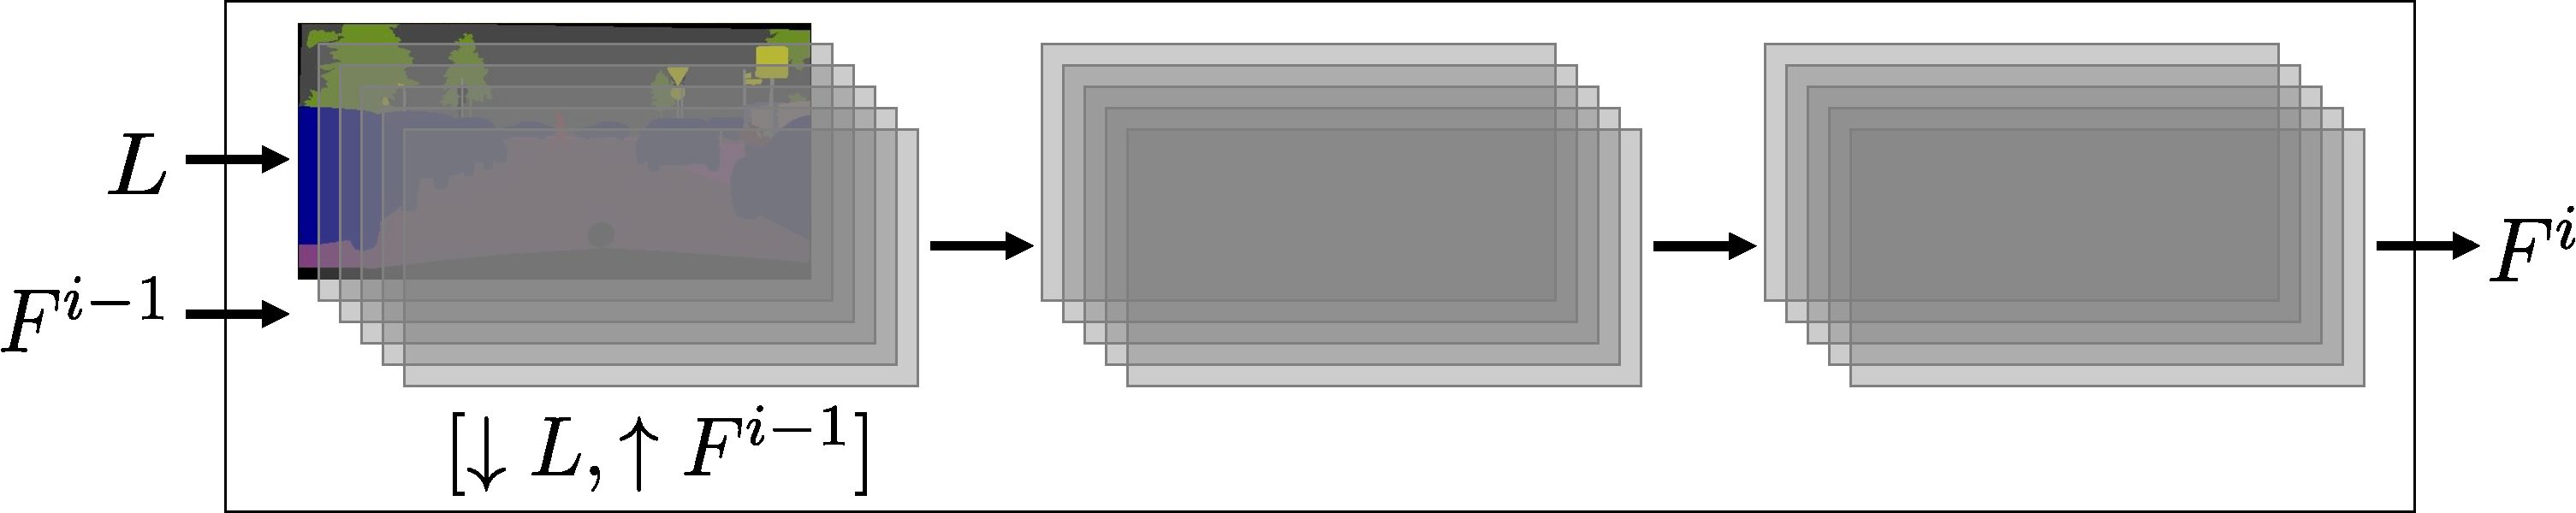
\includegraphics[width=1\linewidth]{figures/diagram2.pdf}
  \caption{A single refinement module.}
\label{fig:module}
\vspace{-1mm}
\end{figure}


\subsection{Architecture}
\label{sec:architecture}

The Cascaded Refinement Network (CRN) is a cascade of refinement modules. Each module $M^i$ operates at a given resolution. In our implementation, the resolution of the first module ($M^0$) is $4\timess 8$. Resolution is doubled between consecutive modules (from $M^{i-1}$ to $M^i$). Let $w_i \timess h_i$ be the resolution of module $i$.

The first module, $M^0$, receives the semantic layout $L$ as input (downsampled to $w_0 \timess h_0$) and produces a feature layer $F^0$ at resolution $w_0 \timess h_0$ as output. All other modules $M^i$ (for ${i\ne 0}$) are structurally identical: $M^i$ receives a concatenation of the layout $L$ (downsampled to $w_i \timess h_i$) and the feature layer $F^{i-1}$ (upsampled to $w_i \timess h_i$) as input, and produces feature layer $F^i$ as output. We denote the number of feature maps in $F^i$ by $d_i$.

Each module $M^i$ consists of three feature layers: the input layer, an intermediate layer, and the output layer. This is illustrated in Figure~\ref{fig:module}. The input layer has dimensionality ${w_i \timess h_i \timess (d_{i-1}+c)}$ and is a concatenation of the downsampled semantic layout $L$ ($c$ channels) and a bilinearly upsampled feature layer $F^{i-1}$ ($d_{i-1}$ channels). Note that we do not use upconvolutions because upconvolutions tend to introduce characteristic artifacts~\cite{Odena2016}.
%In our experiments plain bilinear upsampling avoided the artifacts and.
The intermediate layer and the output layer both have dimensionality $w_i \timess h_i \timess d_i$. Each layer is followed by $3\timess 3$ convolutions, layer normalization~\cite{Ba2016}, and LReLU nonlinearity~\cite{Maas2013}.
%Layer normalization is used because it stabilizes training.
% and (unlike batch normalization) supports training with a single example per iteration.
%Due to the high memory footprint of our model, we train with a single image per iteration.
%, and layer normalization is well-suited to such training regimes.

The output layer $F^{\bar\imath}$ of the final module $M^{\bar\imath}$ is not followed by normalization or nonlinearity. Instead, a linear projection ($1\timess 1$ convolution) is applied to map $F^{\bar\imath}$ (dimensionality ${w_{\bar\imath} \timess h_{\bar\imath} \timess d_{\bar\imath}}$) to the output color image (dimensionality ${w_{\bar\imath} \timess h_{\bar\imath} \timess 3}$).
The total number of refinement modules in a cascade depends on the output resolution. For our main experiments on the high-resolution Cityscapes dataset, the number of modules is 9, accounting for a resolution increase from $4\timess 8$ to $1024 \timess 2048$.
For the number of feature maps $d_i$, we use 1024 for $i = 0..4$, 512 for $i=5,6$, 128 for $i=7$, and 32 for $i=8$.



%After the last module, which outputs a feature layer $F^{\bar\imath}$ of size ${w_{\bar\imath} \timess h_{\bar\imath} \timess d_{\bar\imath}}$,

%\vladlen{Talk about the number of feature maps in each module, $d_i$.}

%Our network is constructed recursively, illustrated in Figure \ref{fig:diagram}. The basic component in the network is a feature extraction function $f$ that transforms an $m\timess n\timess c$ semantic layout $L$ into an $m\times n\times w$ feature map $f(L)$, where $w$ is the number of feature channels. To compute $f(L)$,  we first compute $f(L')$, features at a lower resolution, where $L'$ a downsampled semantic layout. Next, we combine $L$ and the coarse feature map $f(L')$ as the input to the refinement module which generates an $m\timess n\timess w$ feature map as $f(L)$. At the end, we can simply apply $1\timess 1$ convolutions to $f(L)$ to synthesize an $m\timess n \timess 3$ image as $g(L;\theta)$. As the exit to the recursion, when $L$ is at a low resolution (e.g. 4p), we simply use $L$ as the input for refinement without computing $f(L')$.

%In the refinement module, we apply bilinear upsampling to $f(L')$ so that it can be concatenated with $L$. Up convolutions are used because up convolutions can introduce checkboard artifacts \cite{Odena2016}. Together with $L$ and the bilinearly upsampled $f(L')$ as input, the refinement module applies $3\timess 3$ convolutions followed by layer normalization \cite{Ba2016} and leaky rectified units \cite{Maas2013}. Such a step is repeated twice to strengthen the refinement capability. We use layer normalization as it stablizes training and allows training with one image per iteration. Note that we are training with high-resolution images in GPU and we can only afford training one image per iteration.

%Our network is designed in a way to have feature maps with consistent structure.
%Our network starts with the semantic layout downsampled to $4$p as given. Following $3 \timess 3$ convolutions, layer normalization \cite{Ba2016}, and Leaky ReLU \cite{Maas2013} twice as refinement steps to generate feature maps at $4$p. Then the feature map is upsampled to $8$p, and then combined with the semantic layout downsmapled to $8$p as the input to next resolution. Similarly, the same type of refinement steps are performed. At the end, we generate feature maps at full resolution. To generate final output images, we simply apply $1 \timess 1$ convolutions to produce a three-channel feature maps as the output image.


\subsection{Training}

The CRN is trained in a supervised fashion on a semantic segmentation dataset $\dD = \{(I,L)\}$. A semantic layout $L$ is used as input and the corresponding color image $I$ as output. This can be thought of as ``inverse semantic segmentation''. It is an underconstrained one-to-many inverse problem. We will generally refer to $I$ as a ``reference image'' rather than ``ground truth'', since many valid photographic images could have yielded the same semantic layout.

%which contains pairs of a color image $I$ and semantic layout $L$. In semantic segmentation, we commpute a mapping from $I$ to the ground truth $L$. In this task, we are solving the inverse semantic segmentation problem, finding a mapping from $L$ to a reference $I$. We call $I$ is a reference image instead of ground truth because there is no unique ground truth in this problem.

Given the underconstrained nature of the problem, using an appropriate loss function is critical, as observed in prior work on image synthesis. Simply comparing the pixel colors of the synthesized image and the reference image could severely penalize perfectly realistic outputs. For example, synthesizing a white car instead of a black car would induce a very high loss. Instead we adopt the ``content representation'' of Gatys et al.~\cite{Gatys2016}, also referred to as a perceptual loss or feature matching~\cite{Bruna2016,DosovitskiyBrox2016,Johnson2016,Ledig2016,Nguyen2016,Nguyen2017}. The basic idea is to match activations in a visual perception network that is applied to the synthesized image and separately to the reference image.

Let $\Phi$ be a trained visual perception network (we use VGG-19~\cite{SimonyanZisserman2015}). Layers in the network represent an image at increasing levels of abstraction: from edges and colors to objects and categories.
%Thus a white car and a black car of the same shape may differ in low-level activations but will match in higher layers.
Matching both lower-layer and higher-layer activations in the perception network guides the synthesis network to learn both fine-grained details and more global part arrangement.
%The trained networks successfully memorize training images while maintaining generalization ability.
%Due to the high memory footprint of our model, we train with a single image per iteration.

Let $\{\Phi_l\}$ be a collection of layers in the network $\Phi$, such that $\Phi_0$ denotes the input image. Each layer is a three-dimensional tensor.
%Abusing notation, we let $\Phi_0$ denote the input image.
For a training pair ${(I,L) \in \dD}$, our loss is
\begin{equation}
\lL_{I,L}(\theta) = \sum_l{\lambda_l\| \Phi_l(I)-\Phi_l(g(L;\theta))\|_1}.
\label{eq:loss}
\end{equation}
Here $g$ is the image synthesis network being trained and $\theta$ is the set of parameters of this network. The hyperparameters $\{\lambda_l\}$ balance the contribution of each layer $l$ to the loss.

%Designing an appropriate loss for training is critical in our model. Simply comparing the synthesized image and the reference image in color space is a bad idea. For example, if the network synthesizes a white car but the reference image is a black car, the loss will be huge, but we should not penalize too much just because they are very different in color.
%We found that the content loss \cite{Gatys2016} fits our purpose. This loss allows measuring the distance between two images in feature spaces from low-levels (color, edges) to high-levels (semantic).  The distance of a white car and a black one in low-level feature space can be large but is small in the high-level features as they have similar semantic meaning. Low-level features are also needed to memorize fine-grained details. Our loss allows the network to memorize training images while maintaining generalization ability.

%We predefine some feature extraction functions $\{\Phi_l\}$ (e.g. VGG layers) where each $\Phi_l$ maps an image to a feature map. Then our training procedure is to minimize the average content loss for each $(L,I)\in \dD$:
%$$
%\lL(I,L;\theta)=\sum_l{\lambda_l\| \Phi_l(I)-\Phi_l(g(L;\theta))\|_1},
%$$
%where $\{\lambda_l\}$ are the hyperparamters to balance the contribution in each term and $\theta$ is parameters in the convolutions in the network.

For layers $\Phi_l$ ($l\! \ge\! 1$) we use `conv1\_2', `conv2\_2', `conv3\_2', `conv4\_2', and `conv5\_2' in VGG-19~\cite{SimonyanZisserman2015}. The hyperparameters $\{\lambda_l\}$ are set automatically. They are initialized to the inverse of the number of elements in each layer. After 100 epochs, $\{\lambda_l\}$ are rescaled to normalize the expected contribution of each term ${\| \Phi_l(I)-\Phi_l(g(L;\theta))\|_1}$ to the loss.

%We use VGG-19 \cite{SimonyanZisserman2015} to extract features. Each layer in VGG-19 in the network defines features at certain level from low levels to high levels. We use the input layer as well as the "conv1\_2", "conv2\_2", "conv3\_2", "conv4\_2", "conv5\_2" layers for as $\{\Phi_l\}$. This set of features ranges from low levels to high levels. To choose proper $\{\lambda_l\}$, we initial $\lambda_l$ with the inverse of the number of elements in $\Phi_l$ and then train for a number of epoches. Given some training statistics, we can rescale $\{\lambda_l\}$ so that each term $\| \Phi_l(I)-\Phi_l(f(L;\theta))\|$ has similar contribution in the loss.

%Our network architecture also enables efficient training. Instead of training for the whole model directly, we can pretrain a model for 256p-resolution images, then finetune for images at 512p and 1024p resolutions. It takes one to two three weeks for training.


\subsection{Synthesizing a diverse collection}
\label{sec:diversity}

The architecture and training procedure described so far synthesize a single image for a given input $L$. In our experiments this already yields good results.
% and we use this procedure for the quantitative experiments reported in Section~\ref{}
However, since a given semantic layout can correspond to many images, it also makes sense to generate a diverse set of images as output.
%A car can be black, red, or white, and can face forward or backwards.
Conditional synthesis of diverse images can be approached as a stochastic process~\cite{Nguyen2017}. We take a different tack and modify the network to emit a collection of images in one shot, with a modified loss that encourages diversity within the collection.

%Inherently, there is no unique "ground-truth" image that conforms to the given semantic layout. For example, given a semantic layout of a car, we can synthesize a black, red, or white car and it might be facing front or back. Our CRN is able to generate diverse images explicitly.

Specifically, we change the number of output channels from $3$ to $3k$, where $k$ is the desired number of images. Each consecutive 3-tuple of channels forms an image. Now consider the loss. If loss (\ref{eq:loss}) is applied independently to each output image, the $k$ synthesized images will be identical. Our first modification is to consider the set of $k$ outputs together and define the loss of the whole collection in terms of the \emph{best} synthesized image. Let $g_u(L;\theta)$ be the $u^{\text{th}}$ image in the synthesized collection. Our first version of the modified loss is based on the hindsight loss developed for multiple choice learning~\cite{Guzman-Rivera2012}:
\begin{equation}
\min_u{\sum_l{\lambda_l\| \Phi_l(I)-\Phi_l(g_u(L;\theta))\|_1}}.
\label{eq:loss-diverse1}
\end{equation}
By considering only the best synthesized image, this loss encourages the network to spread its bets and cover the space of images that conform to the input semantic layout. The loss is structurally akin to the $k$-means clustering objective, which only considers the closest centroid to each datapoint and thus encourages the centroids to spread and cover the dataset.
%This loss encourage diversity in the output images, because having the same output images does not help reduce the loss. We only need one of them for comparison. This loss is similar to k-means clustering loss and the centroid is unlikely to collide.

%In order to generate $k$ images from our network, we simply change the number of feature channels in the final layer from $3$ to $3k$. Every three feature maps can form an image, totally $k$ images. With $k$ output images, we also need to adjust our loss function. We need a loss function that measures the distance between a reference image in the training data and $k$ generated images. Intuitively, we should not penalize as long as the reference is close to one of $k$ output images. Let $g_u(L,\theta)$ denote the $u$-th image the network synthesize. The loss $\lL(I,L;\theta)$ for our CRN with $k$ output images would become,
%\begin{equation}
%\min_u{\sum_l{\lambda_l\| \Phi_l(I)-\Phi_l(g_u(L;\theta))\|_1}}.
%\label{eqn:diversity_loss_1}
%\end{equation}
%This loss encourage diversity in the output images, because having the same output images does not help reduce the loss. We only need one of them for comparison. This loss is similar to k-means clustering loss and the centroid is unlikely to collide.

We further build on this idea and formulate a loss that considers a virtual collection of up to $k^c$ images. (Recall that $c$ is the number of semantic classes.) Specifically, for each semantic class $p$, let $L_p$ denote the corresponding channel $L(\cdot,\cdot,p)$ in the input label map. We now define a more powerful diversity loss as
\begin{equation}
\resizebox{.9\hsize}{!}{$\displaystyle{
\sum_{p=1}^c{\min_u{\sum_l{\lambda_l\sum_j \big\|L_p^l \odot \big(\Phi_l^j(I)-\Phi_l^j(g_u(L;\theta))\big)\big\|_1}}},
}$}
\label{eq:loss-diverse2}
\end{equation}
where $\Phi_l^j$ is the $j^{\text{th}}$ feature map in $\Phi_l$, $L_p^l$ is the mask $L_p$ downsampled to match the resolution of $\Phi_l$, and $\odot$ is the Hadamard product. This loss in effect constructs a virtual image by adaptively taking the best synthesized content for each semantic class from the whole collection, and scoring the collection based on this assembled image.
%We will demonstrate the effect of this loss qualitatively in our experiments.

%Furthermore, the loss (\ref{eqn:diversity_loss_1}) can be improved as we could construct up to $k^c$ different images from just $k$ output images: for each class out of $c$ semantic classes, we can choose one $k$ images to fill the content of the regions of that class. However, it is computationally intractable to explicit compute $k^c$ images.
%In fact, computing the loss between the reference image and $k^c$ constructed images can be computed efficiently, semantic classes are sperable during construction. Intuitively, as long as one of $k$ images has similar output with the reference image in the areas of that semantic class, we should not penalize. Therefore, we can have a loss that sum up the per-class losses:
%$$
%\sum_{p=1}^c{\min_u{\sum_l{\lambda_l\|mask(L,p,l) \odot \left(\Phi_l(I)-\Phi_l(g_u(L;\theta))\right)\|_1}}},
%$$
%where $mask(L,p,l)$ is a mask image $M$ with the same shape of $\Phi_l$. Suppose $M$ has shape $m'\timess n' \timess w'$ and let $L'$ be the resized semantic layout of $L$ with size $m'\timess n'\timess c$. Then $M_{i,j,z}=L'_{i,j,p}$ for all $z$. $M$ eliminates penalty in regions where the semantic class is not $p$.

\begin{comment}

      POTENTIAL MATERIAL FOR THE SUPPLEMENT:

      \begin{figure}[h]
        \centering
        \begin{tabular}{@{}c@{\hspace{0.5mm}}c@{}}
        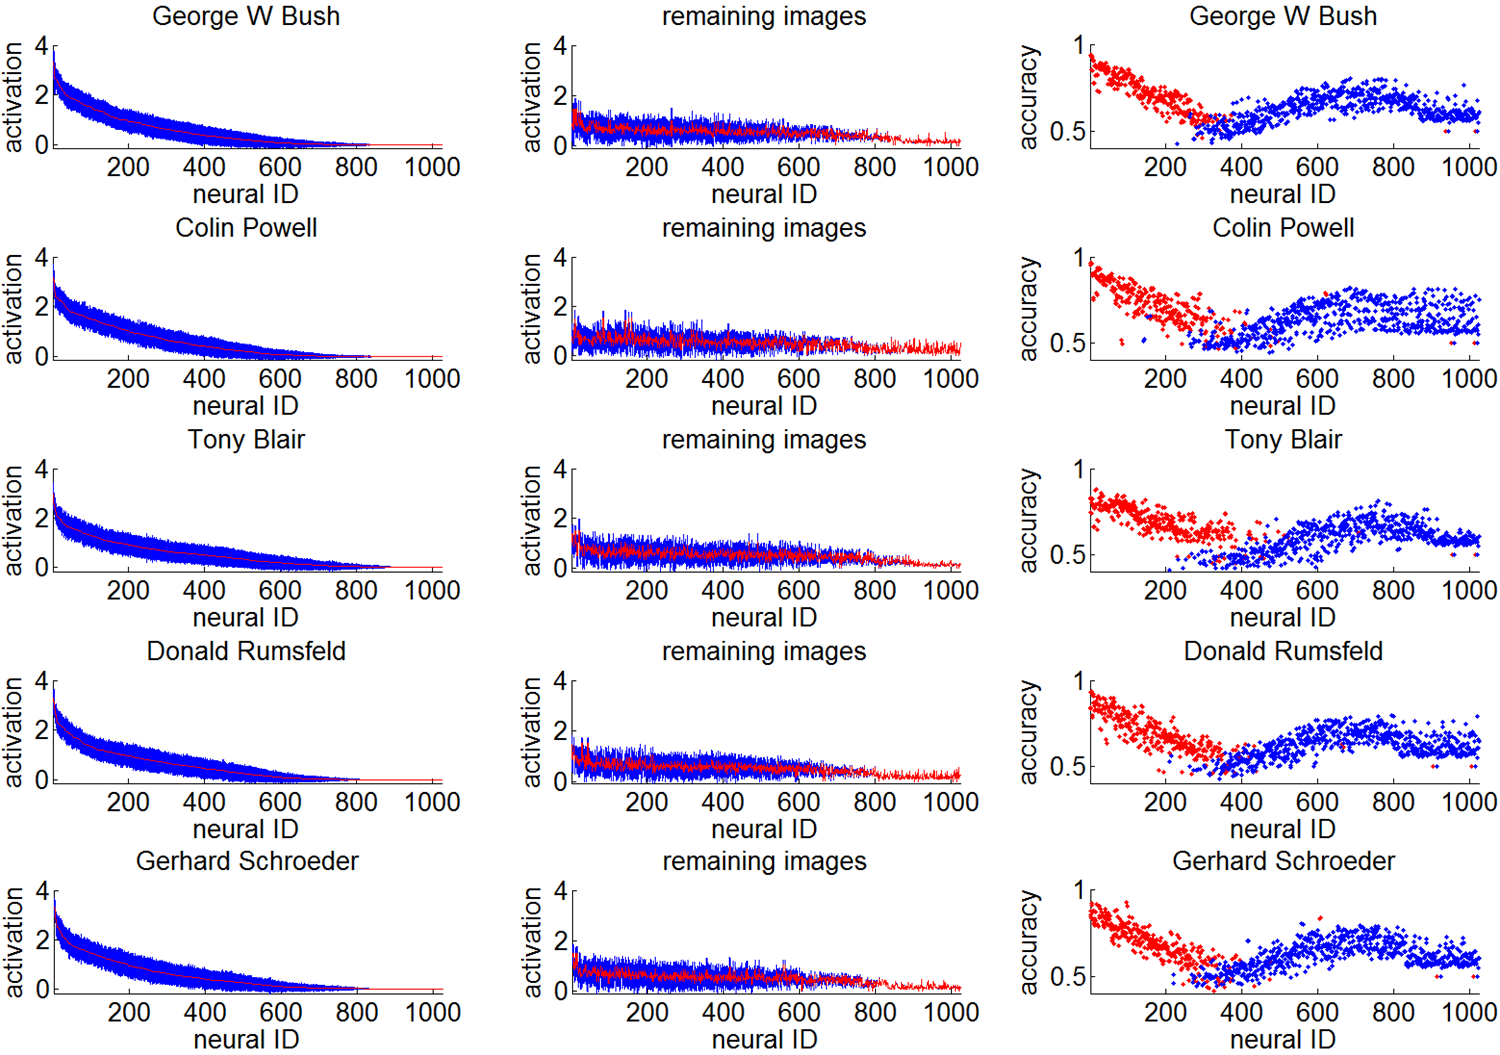
\includegraphics[width=0.235\textwidth]{figures/diversity/1.png}&
        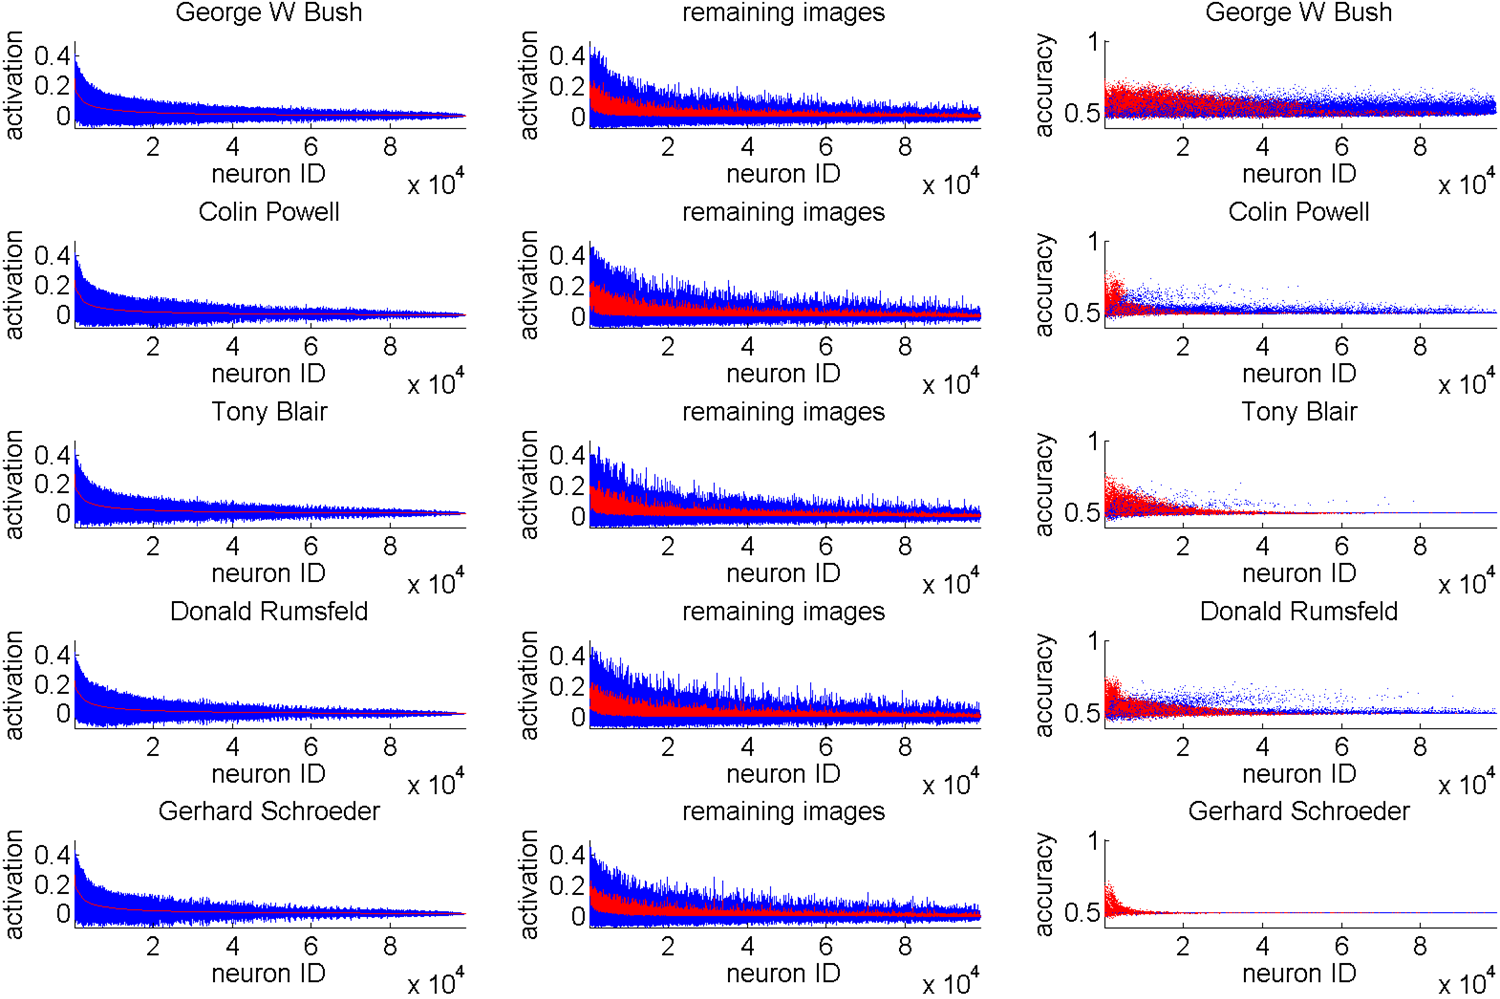
\includegraphics[width=0.235\textwidth]{figures/diversity/2.png}\\
        Output A& Output B\\
        \end{tabular}
        \caption{diversity.}
      \label{fig:diversity}
      \end{figure}

\end{comment}
